\documentclass[14pt]{beamer}
\title{WEB :: HTML}
\author[TS]{TalentSprint}
\institute[L\&D]{Licensed To Skill}
\usefonttheme{serif}
\usecolortheme{orchid}
\usepackage{bookman}
\usepackage{multirow}
\usepackage{fancybox}
\usepackage[percent]{overpic}
\usepackage{hyperref}
\usepackage[T1]{fontenc}
\usepackage{graphicx}
\usepackage{listings}
\graphicspath{{./../Images/}}
\usepackage{tikz}
\usepackage{soul}
\usepackage{color}
\beamertemplateballitem
\usebackgroundtemplate{
\includegraphics[width=\paperwidth]{TS-XP-Logo.jpg}}
\lstset{language=html, numbers=left, numbers=none, basicstyle=\footnotesize, numberstyle=\tiny,  numbersep=10pt, showstringspaces=false, breaklines=true,keepspaces=true, columns=flexible}
\begin{document}

\begin{frame}
  \titlepage
\end{frame}

\begin{frame}{HTML Basics}
The content in this presentation is aimed at teaching  learners to:
  \begin{itemize}
  \item Create web pages using frames
  \item Insert HTML input controls in the webpage
  \end{itemize}
\end{frame}

\begin{frame}{Frame and Form Controls}
\begin{figure}[H]
\centering
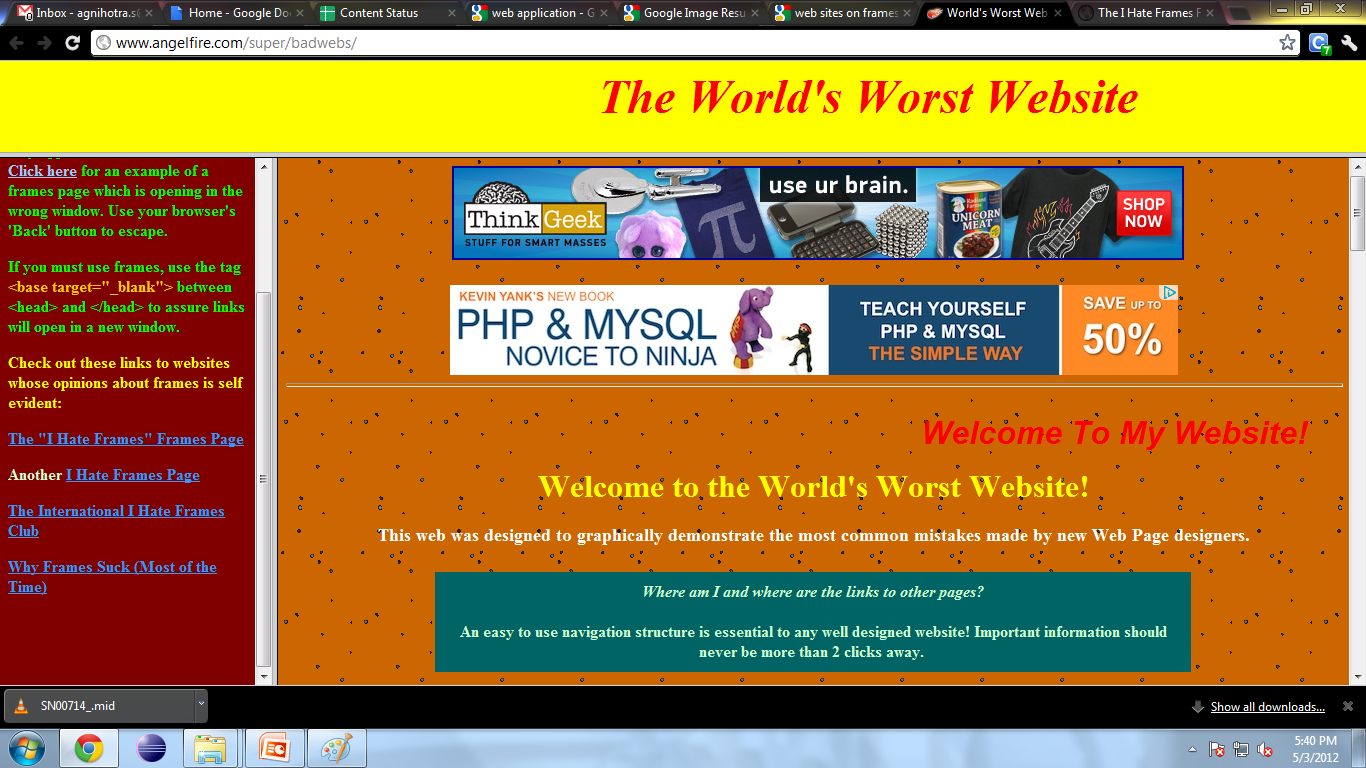
\includegraphics[scale=.2]{frame-form-control.png}
\end{figure}
\end{frame}

\begin{frame}{Frame and Form Controls}
\begin{figure}[H]
\centering
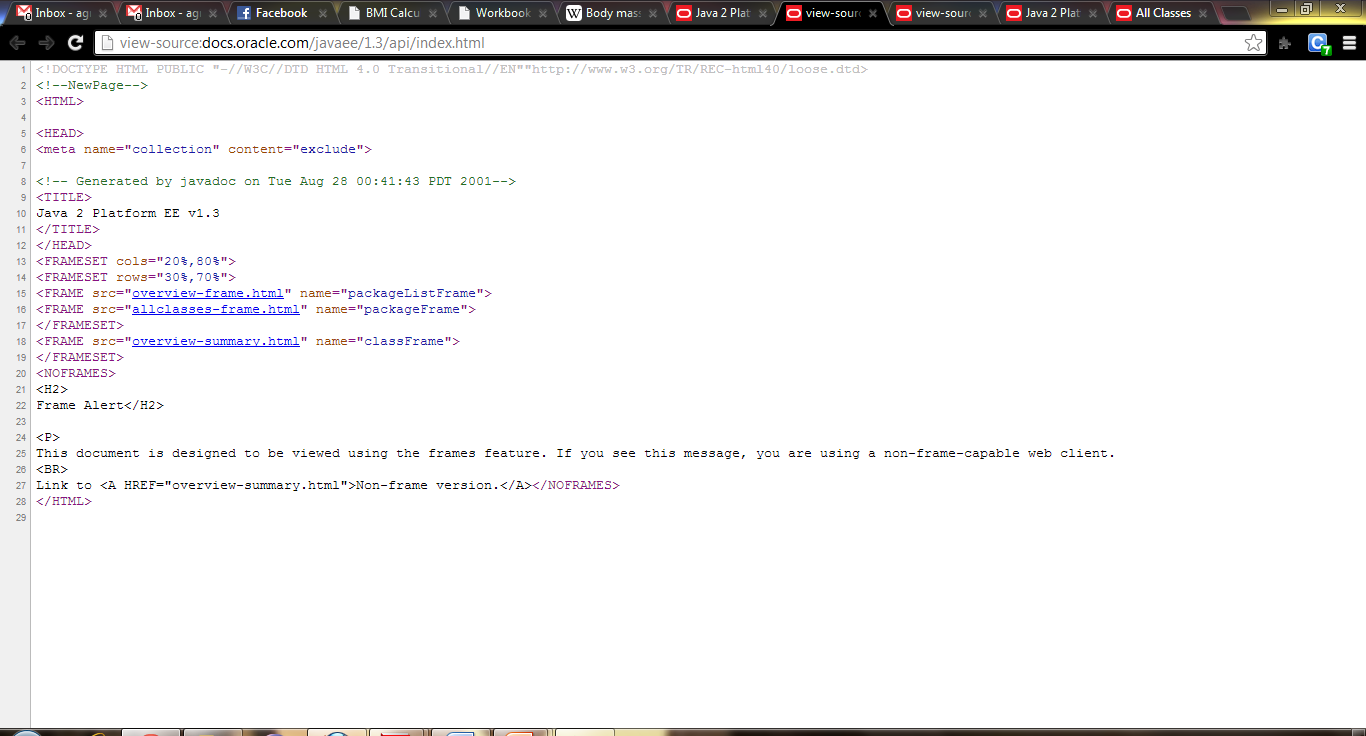
\includegraphics[scale=.2]{frame-form-control2.png}
\end{figure}
\end{frame}

\begin{frame}{Frame and Form Controls}
\begin{figure}[H]
\centering
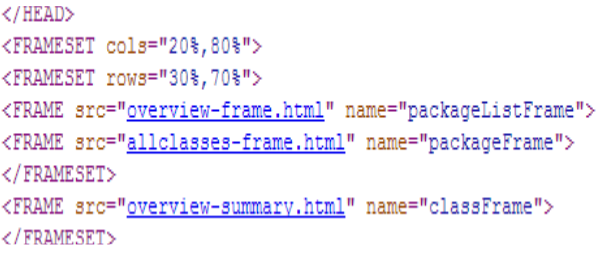
\includegraphics[scale=.5]{frame-form-control3.png}
\end{figure}
\end{frame}

\begin{frame}{Frame and Form Controls}
\begin{figure}[H]
\centering
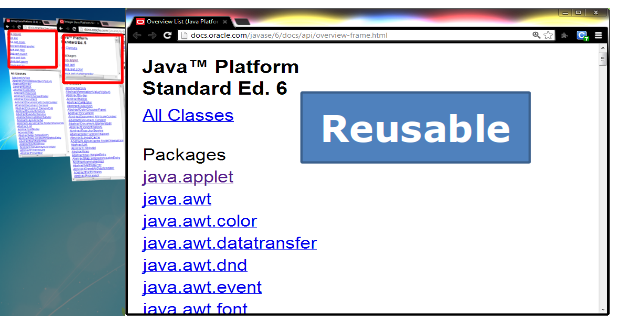
\includegraphics[scale=.5]{frame-form-control4.png}
\end{figure}
\end{frame}

\begin{frame}{Frame and Form Controls}
\begin{figure}[H]
\centering
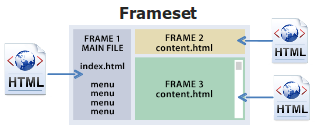
\includegraphics[width=5cm, height=2cm]{frameset.png}
\end{figure}
\begin{itemize}
 \item Divides the screen into separate frames.
 \item Each frame can contain an HTML document.
 \item A file or HTML Document that specifies how the screen is divided into frames is called a frameset.
\end{itemize}
\end{frame}

\begin{frame}{Frame and Form Controls}
If you want to make a homepage that uses frames, you should: 
\begin{itemize}
 \item Create an HTML document with the frameset.
 \item Create the normal HTML documents that should be loaded into each of these frames.
\end{itemize}
\end{frame}

\begin{frame}{Frame and Form Controls}
\textbf{Creating Frameset}

\vspace{1pc}
\small
A frameset is simply an HTML document that tells the browser how to divide the screen into split windows.

\begin{minipage}{5cm}
\begin{block}{Example}
\lstinline!<frameset cols = ``120, *''>!

\lstinline!</frameset>!
\end{block}
\end{minipage}
\quad
\begin{minipage}{4cm}

\includegraphics[scale=.4]{frameset-example.png}
\end{minipage}
`cols'  is an attribute to divide the window into two columns 

The left being 120 pixels and the right using the rest of the screen (indicated by the *).
\end{frame}

\begin{frame}{Frame and Form Controls}
Creating Frameset
\begin{itemize}
 \item The values of rows and columns can be in pixels value or can be percentage value of screen space.
 \item Number of rows or columns seperated with commas, decides the number of frames in the page.
 \item Frameset  tag will not work in $<$body$>$ tag.
\end{itemize}
\end{frame}

\begin{frame}{Frame and Form Controls}
Defining Frame
\begin{itemize}
 \item The $<$frame$>$ tag defines one particular window (or frame) within a frameset.
 \item You can add default pages to the frames by using the src attribute of the frame tag.
 \item You can add names to each frame by using the name attribute. 
\end{itemize}
\end{frame}

\begin{frame}{Frame and Form Controls}
Defining Frame
\begin{itemize}
 \item Name attribute allow us to display a link in one frame and open the page in another frame.

 Example:
 
\begin{minipage}{5cm}
\begin{figure}[H]
 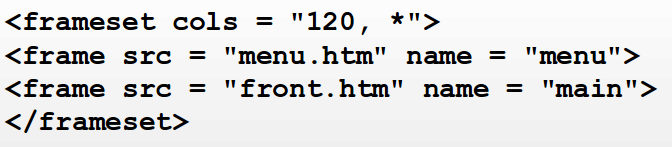
\includegraphics[scale=.29]{define-frame1.png}
\end{figure}
\end{minipage}
\quad
\begin{minipage}{4cm}
\begin{figure}[H]
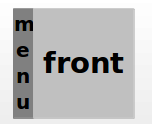
\includegraphics[scale=.3]{define-frame2.png}
\end{figure}
\end{minipage}
\item Comma separated values of row/cols in frameset will maps to the list of frames defined in frameset respectively.
\end{itemize}
\end{frame}

\begin{frame}{Frame and Form Controls}
Attributes for Frame and Frameset

\vspace{1pc}
\begin{enumerate}
 \item \textbf{frameborder} Specifies whether or not to display a border around a frame.
 \begin{itemize}
  \item `0' means no border
  \item Any numerical value other than `0' shows the border
 \end{itemize}
\item \textbf{width} Specifies the width of the border in pixels/percentage
\end{enumerate}
\end{frame}

\begin{frame}{Frame and Form Controls}
\begin{enumerate}
\setcounter{enumi}{2}
 \item \textbf{noresize} Specifies that a frame is not resizable
 \item \textbf{scrolling} Specifies whether or not to display scrollbars in a frame.
 \begin{itemize}
  \item Values are yes, no and auto
 \end{itemize}
\end{enumerate}
\end{frame}

\begin{frame}[fragile]{Frame and Form Controls}
\begin{center}
 \begin{tabular}{l l l}
  \multirow{6}{*}{\rotatebox{90}{Menupage.html}} & Welcomepage.html & 
\includegraphics[scale=.3]{try-it.png}\\
   & & \\
   & & \\
   & & \\
   & & \\
   & Bottombanner.html &\\
 \end{tabular}
\end{center}
\pause
\begin{lstlisting}
<frameset cols = ``120, *'' scrolling = auto>
    <frame src = ``Menupage.htm'' name = ``menu'' noresize>
    <frameset rows = ``*, 50'' frameborder = 1 border = 10> 
        <frame src = ``Welcomepage.htm'' name = ``main''>
        <frame src = ``Bottombanner.htm'' name = ``bottom''>
    </frameset> 
</frameset>
\end{lstlisting}
\end{frame}
\begin{frame}{Frame and Form Controls}
\begin{figure}[H]
\centering
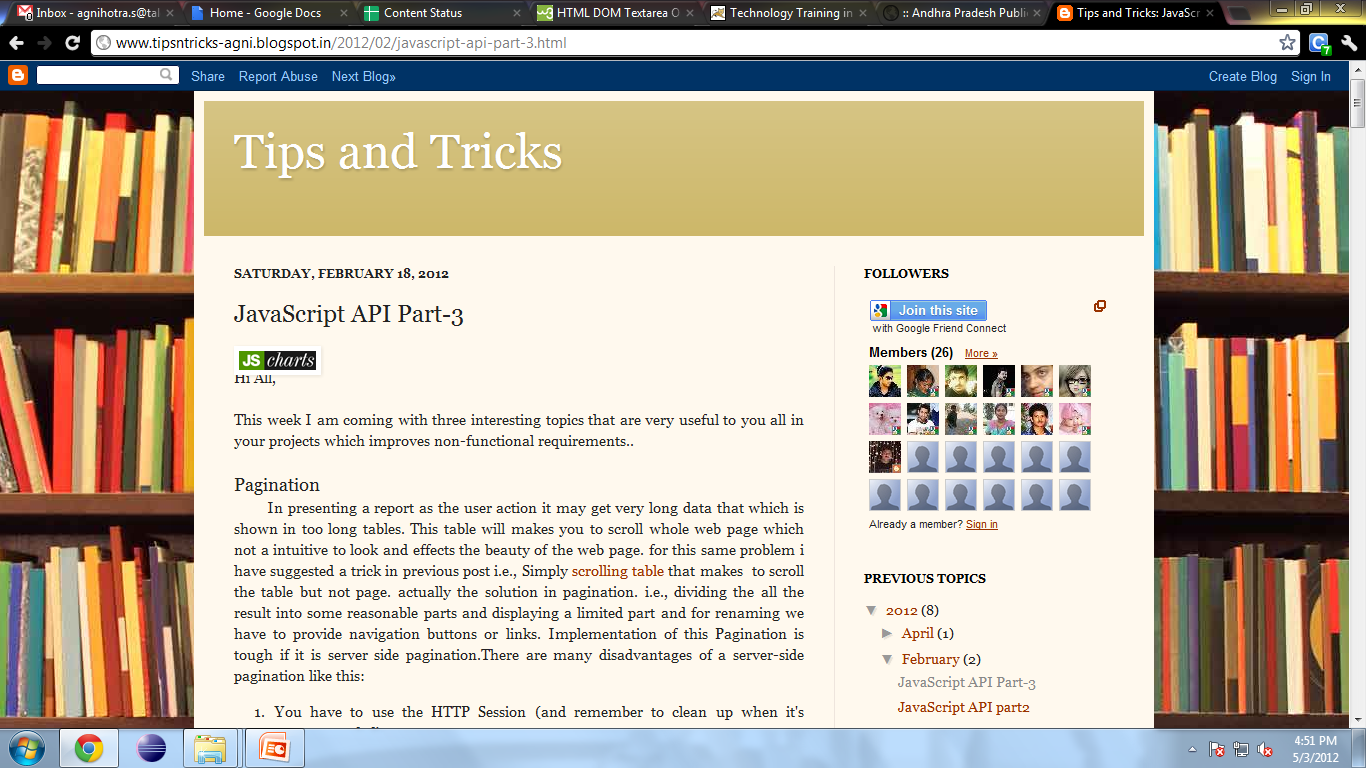
\includegraphics[scale=.2]{tips-tricks.png}
\end{figure}
\end{frame}

\begin{frame}{Frame and Form Controls}
\small
\begin{overpic}[scale=.2]{frameset-working-example.png}
\put (20,15) {\colorbox{green}{Data (Input) Acceptance }}
\end{overpic}
\end{frame}

\begin{frame}{Frame and Form Controls}
What after Acceptance?

\begin{figure}[H]
\centering
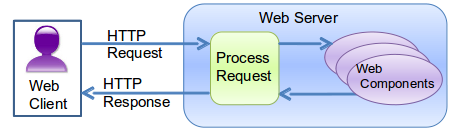
\includegraphics[scale=.4]{input-acceptance.png}
\end{figure}
\begin{enumerate}
 \item Validates Inputs
 \begin{itemize}
  \item Accepting only numbers
  \item Mandatory Fields 
  \item Passwords matches .. Etc
 \end{itemize}
 For all the above we need validation at Client Side 
\end{enumerate}
\end{frame}

\begin{frame}{Frame and Form Controls}
\begin{enumerate}
\setcounter{enumi}{1}
 \item Sends data for further processing like Insert, Updates and Calculates Computational Tasks by:
 \begin{itemize}
  \item Generates the REQUEST 
  \item Transfers the Data to the Sever  
 \end{itemize}
 \item Server Process the request and responds back as necessary.
\end{enumerate}
\end{frame}

\begin{frame}{Frame and Form Controls}
\small
\begin{tabular}{p{3cm} p{2cm} p{2cm} p{2cm}}
 Challan No. / ReferenceID* & \framebox[2cm]{} &  Date Of Birth*& \framebox[2cm]{} \\
 Journal No* & \framebox[2cm]{} & Date Of Payment*& \framebox[2cm]{} \\
 & \colorbox{orange}{submit} & &\\
\end{tabular}
\begin{itemize}
 \item A form is an area that can contain form fields.
 \item Form fields are objects that allow the visitor/user to enter information.
 \item When the user clicks the submit button, the content of the form is usually sent to a program that runs on the server.
\end{itemize}
\end{frame}

\begin{frame}{Frame and Form Controls}
Form Tag

\small
\begin{itemize}
 \item \lstinline!<form>! tells the browser where the form starts and ends.
 \item Includes all kind of HTML tags between \lstinline!<form>! and \lstinline!<form>!.
 \item To specify where to send the content, we have to add these properties to the \lstinline!<form>! tag
 \begin{itemize}
  \item action = <url> 
  \item method = < POST | GET >
 \end{itemize}
The address is the url of the cgi script where the content should be sent to.
\item POST and GET methods are simply two different methods of submitting data to the script.
\end{itemize}
\end{frame}

\begin{frame}[fragile]{Frame and Form Controls}
Form Tag Example
\begin{lstlisting}
<html>
    <head>
        <title>My Page</title>
    </head>
    <body>
        <!-- Here goes HTML -->
        <form method = ``post'' action = ``http://www.echoecho.com/cgi-bin/formmail.cgi''>
            <!-- Here goes form fields and HTML -->
        </form> 
        <!-- Here goes HTML -->
    </body>
</html> 
\end{lstlisting}
\end{frame}

\begin{frame}{Frame and Form Controls}
\small
\def\arraystretch{1.5}
\begin{tabular}{ | p{2cm} | p{3cm} | p{4cm} |}
\hline
\textbf{Form Field} & \textbf{UI Presentation} & \textbf{HTML Code} \\ \hline
Text Filed & \framebox[2cm]{}& \lstinline!<input type = ``text''>! \\ \hline
Password & \framebox[2cm]{} & \lstinline!<input type = ``password''>! \\ \hline
Hidden Field & & \lstinline!<input type = ``hidden''>! \\ \hline
Text Area & \ovalbox{\begin{minipage}{2.5cm} \vspace{4pc}\hspace{1pc}\end{minipage}} & \lstinline!<textarea width = 20 height = 5> </textarea>! \\ \hline
\end{tabular}
\end{frame}

\begin{frame}{Frame and Form Controls}
Form Submission

\vspace{1pc}
This is what may happens when the form is submitted:
\begin{itemize}
 \item Performs the Client Side Scripting.
 \item Generates HTTP Request according to Specifications (GET/POST).
 \item Transfer the form data to the server side scripting.
 \item Server process the request to perform the particular task.
\end{itemize}
\end{frame}

\begin{frame}{Frame and Form Controls}
Input Attributes
\begin{center}
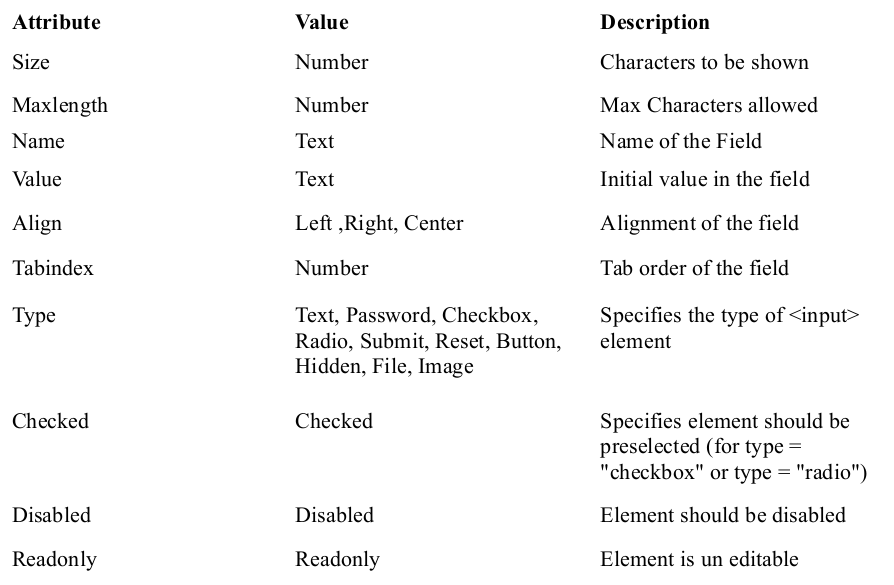
\includegraphics[scale=.3]{input-attributes.png} 
\end{center}
\end{frame}

\begin{frame}{Fram and Form Controls}
Text Area
\begin{itemize}
 \item Text areas are the text fields that can span several lines
 \item Text areas are not defined with an \lstinline!<input>! tag
 \item Everything written between \lstinline!<textarea>! and \lstinline!<textarea>! tags will be presented in the text area box.
\end{itemize}
\end{frame}

\begin{frame}{Frame and Form Controls}
Text Area

\vspace{1pc}
\begin{tabular}{|p{2.5cm} | p{2cm} | p{4cm} |}
 \hline
 \textbf{Attribute} & \textbf{Value} & \textbf{Description} \\ \hline
 Rows & Number & Rows in the field \\ \hline
 Cols & Number & Columns in the field \\ \hline
 Name & Text & Name of the field \\ \hline
 Tabindex & Number & Tab Order of the field \\ \hline
 Wrap & & Turns off line breaking  \\ \hline
 \end{tabular}
\end{frame}

\begin{frame}{Frame and Form Controls}
Dropdown Menu

\vspace{.5pc}
\begin{itemize}
 \item It serves the same purpose as:
 \begin{itemize}
 \item Radio buttons (one selection only)
 \item Check boxes (multiple selections allowed)
 \end{itemize}
 \item It has combine  usage of \lstinline!<select>! and \lstinline!<option>!. Both tags have an opening and a closing tag
 \end{itemize}
Disadvantage is that all options are not visible unless the menu is selected.
\end{frame}

\begin{frame}{Frame and Form Controls}
Dropdown Menu

\vspace{.5pc}
\begin{tabular}{|p{2.5cm}|p{2.5cm}|p{4cm}|}
\hline 
\textbf{Attribute} & \textbf{Value} & \textbf{Description} \\ \hline
Name  & Text & Name of the element \\ \hline
Size & Number & No. of options to display \\ \hline
Multiple & Multiple & Allows multiple selection \\ \hline
Value for option tag & Text & Value of the selection \\ \hline
\end{tabular}
\end{frame}

\begin{frame}{Frame and Form Controls}
\textbf{Buttons}

\vspace{1pc}
Three type of buttons based on input type:
\begin{description}
 \item [Button] Normal button 
 \item [Submit] Button which submits the form
 \item [ Reset] Button which sets the form data to the default values
\end{description}
\end{frame}

\begin{frame}{Frame and Form Controls}
\begin{tabular}{p{8cm} p{2cm}}
Write the code to create a webpage containing the following form: & 
\includegraphics[scale=.25]{try-it.png}  \\
\end{tabular}


\begin{figure}[H]
 \centering
 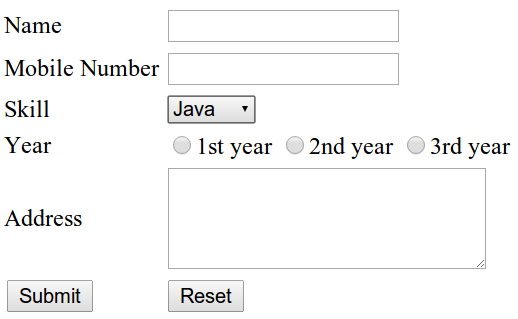
\includegraphics[scale=.4]{exercise-try-it.png}
\end{figure}
\end{frame}

\begin{frame}{Frame and Form Controls}
 \begin{figure}[H]
 \begin{center}
   
\includegraphics[scale=.3]{qa.png}   
 \end{center}
  \end{figure}
\end{frame}

\end{document}
